\documentclass[12pt]{article}
\usepackage{amsmath}
\usepackage{graphicx}
\usepackage{chngpage}
\graphicspath{{./src/}}
\begin{document}
\title{Computer Science M146, Homework 5}
\date{March 15th, 2018}
\author{Michael Wu\\UID: 404751542}
\maketitle

\section*{Problem 1}

\paragraph{a)}

We lose the ordering of the documents, as a document \(D_1=\{a,b,c\}\) is treated as equivalent to the document \(D_2=\{a,c,b\}\). We only
care about the number of words in the document, not the order they appear in.

\paragraph{b)}

\begin{align*}
        \log \operatorname{P}(D_i, y_i) &= \log\left(\left(\operatorname{P}(D_i|y_i=1)\operatorname{P}(y_i=1)\right)^{y_i}
                \left(\operatorname{P}(D_i|y_i=0)\operatorname{P}(y_i=0)\right)^{1-y_i}\right)\\
        &=\log \left(\operatorname{P}(D_i|y_i=1)^{y_i}\theta^{y_i}\operatorname{P}(D_i|y_i=0)^{1-y_i}(1-\theta)^{1-y_i}\right)\\
        &=y_i(\log \theta + \log \operatorname{P}(D_i|y_i=1))\\
        &\qquad+(1-y_i) (\log (1-\theta) + \log \operatorname{P}(D_i|y_i=0))\\
        &=y_i\left(\log \theta + \log \frac{n!}{a_i!b_i!c_i!}\alpha_1^{a_i}\beta_1^{b_i}\gamma_1^{c_i}\right)\\
        &\qquad+(1-y_i) \left(\log(1-\theta)+ \log \frac{n!}{a_i!b_i!c_i!}\alpha_0^{a_i}\beta_0^{b_i}\gamma_0^{c_i}\right)\\
        &=y_i\left(\log \theta + \log \frac{n!}{a_i!b_i!c_i!}+a_i\log\alpha_1+b_i\log\beta_1+c_i\log\gamma_1\right)\\
        &\qquad+(1-y_i) \left(\log(1-\theta)+ \log \frac{n!}{a_i!b_i!c_i!}+a_i\log\alpha_0+b_i\log\beta_0\right.\\
        &\qquad\left.\phantom{\frac{0}{0}}+c_i\log\gamma_0\right)
\end{align*}

\begin{align*}
        \log \operatorname{P}(D_i, y_i) &= \log \frac{n!}{a_i!b_i!c_i!} + y_i(\log \theta +a_i\log\alpha_1+b_i\log\beta_1+c_i\log\gamma_1)\\
        &\qquad+(1-y_i)(\log(1-\theta)+a_i\log\alpha_0+b_i\log\beta_0+c_i\log\gamma_0)
\end{align*}

\paragraph{c)}

We can find the maximum likelihood estimate for each of our parameters by finding
\[\max_{\alpha_1,\beta_1,\gamma_1,\alpha_0,\beta_0,\gamma_0}\sum_{i=1}^m\log \operatorname{P}(D_i, y_i)\]
Our maximum likelihood estimate occurs when
\[\frac{\partial}{\partial \alpha_1}\sum_{i=1}^m\log \operatorname{P}(D_i, y_i)=0\]
Because we are given that \(\alpha_1+\beta_1+\gamma_1=1\), we know that \(\beta_1\) is a function of \(\alpha_1\) and \(\gamma_1\). So we can let
\(\beta_1=1-\alpha_1-\gamma_1\). Taking the partial derivative yields
\begin{align*}
        \frac{\partial}{\partial \alpha_1}\sum_{i=1}^m\log \operatorname{P}(D_i, y_i)&=\frac{\partial}{\partial \alpha_1}\sum_{i=1}^m y_i(a_i\log\alpha_1+b_i\log\beta_1)\\
        &=\frac{\partial}{\partial \alpha_1}\sum_{i=1}^m y_i(a_i\log\alpha_1+b_i\log(1-\alpha_1-\gamma_1))\\
        &=\sum_{i=1}^my_i\left(\frac{a_i}{\alpha_1}-\frac{b_i}{1-\alpha_1-\gamma_1}\right)\\
        &=\sum_{i=1}^my_i(a_i(1-\alpha_1-\gamma_1)-b_i\alpha_1)\\
        &=(1-\gamma_1)\sum_{i=1}^m y_ia_i-\alpha_1\sum_{i=1}^m y_i(a_i+b_i)
\end{align*}
Then we can solve for zero which gives
\[\alpha_1=\frac{\sum_{i=1}^m y_ia_i}{\sum_{i=1}^m y_i(a_i+b_i)}(1-\gamma_1)=C_1(1-\gamma_1)\]
Using the same process with the partial derivative for \(\gamma_1\) yields
\begin{align*}
        \frac{\partial}{\partial \gamma_1}\sum_{i=1}^m\log \operatorname{P}(D_i, y_i)&=\frac{\partial}{\partial \gamma_1}\sum_{i=1}^m y_i(c_i\log\gamma_1+b_i\log\beta_1)\\
        &=\sum_{i=1}^my_i\left(\frac{c_i}{\gamma_1}-\frac{b_i}{1-\alpha_1-\gamma_1}\right)\\
        &=\sum_{i=1}^my_i(c_i(1-\alpha_1-\gamma_1)-b_i\gamma_1)\\
        &=(1-\alpha_1)\sum_{i=1}^m y_ic_i-\gamma_1\sum_{i=1}^m y_i(b_i+c_i)
\end{align*}
Setting this equal to zero gives us
\[\gamma_1=\frac{\sum_{i=1}^m y_ic_i}{\sum_{i=1}^m y_i(b_i+c_i)}(1-\alpha_1)=C_2(1-\alpha_1)\]
and thus
\begin{align*}
        \alpha_1&=\frac{C_1(1-C_2)}{1-C_1C_2}\\
        \beta_1&=\frac{(1-C_1)(1-C_2)}{1-C_1C_2}\\
        \gamma_1&=\frac{C_2(1-C_1)}{1-C_1C_2}
\end{align*}
where
\begin{align*}
        C_1&=\frac{\sum_{i=1}^m y_ia_i}{\sum_{i=1}^m y_i(a_i+b_i)}\\
        C_2&=\frac{\sum_{i=1}^m y_ic_i}{\sum_{i=1}^m y_i(b_i+c_i)}
\end{align*}
Similarly for \(\alpha_0\), \(\beta_0\), and \(\gamma_0\), taking partial derivatives and setting them to zero yields
\begin{align*}
        \alpha_0&=\frac{C_3(1-C_4)}{1-C_3C_4}\\
        \beta_0&=\frac{(1-C_3)(1-C_4)}{1-C_3C_4}\\
        \gamma_0&=\frac{C_4(1-C_3)}{1-C_3C_4}
\end{align*}
where
\begin{align*}
        C_3&=\frac{\sum_{i=1}^m (1-y_i)a_i}{\sum_{i=1}^m (1-y_i)(a_i+b_i)}\\
        C_4&=\frac{\sum_{i=1}^m (1-y_i)c_i}{\sum_{i=1}^m (1-y_i)(b_i+c_i)}
\end{align*}
because of the symmetry of our log likelihood function \(\log \operatorname{P}(D_i, y_i)\). After some algebraic simplification
these values become
\begin{align*}
        \alpha_1&=\frac{\sum_{i=1}^m y_ia_i}{\sum_{i=1}^m y_in}\\
        \beta_1&=\frac{\sum_{i=1}^m y_ib_i}{\sum_{i=1}^m y_in}\\
        \gamma_1&=\frac{\sum_{i=1}^m y_ic_i}{\sum_{i=1}^m y_in}\\
        \alpha_0&=\frac{\sum_{i=1}^m (1-y_i)a_i}{\sum_{i=1}^m (1-y_i)n}\\
        \beta_0&=\frac{\sum_{i=1}^m (1-y_i)b_i}{\sum_{i=1}^m (1-y_i)n}\\
        \gamma_0&=\frac{\sum_{i=1}^m (1-y_i)c_i}{\sum_{i=1}^m (1-y_i)n}
\end{align*}
such that \(\alpha_1\) is the total proportion of \(a\) words in the set of \(D_i\) that have label \(y_i=1\), \(\beta_1\) is the total
proportion of \(b\) words in the set of \(D_i\) that have label \(y_i=1\), \(\gamma_1\) is the total proportion of \(c\) words in the set
of \(D_i\) that have label \(y_i=1\), \(\alpha_0\) is the total proportion of \(a\) words in the set of \(D_i\) that have label \(y_i=0\),
\(\beta_0\) is the total proportion of \(b\) words in the set of \(D_i\) that have label \(y_i=0\), and
\(\gamma_0\) is the total proportion of \(c\) words in the set of \(D_i\) that have label \(y_i=0\).

\section*{Problem 2}

\paragraph{a)}

The two unspecified state transitions are
\begin{align*}
        q_{21}&=\operatorname{P}(q_{t+1}=2|q_t=1)=0\\
        q_{22}&=\operatorname{P}(q_{t+1}=2|q_t=2)=0
\end{align*}
The two unspecified output probabilities are
\begin{align*}
        e_1(B)&=\operatorname{P}(O_t=B|q_t=1)=0.01\\
        e_2(A)&=\operatorname{P}(O_t=A|q_t=2)=0.49
\end{align*}

\paragraph{b)}

We have
\[\operatorname{P}(A)=\pi_1e_1(A)+\pi_2e_2(A)=0.49\times0.99+0.51\times0.49=0.735\]
We also have
\[\operatorname{P}(B)=\pi_1e_1(B)+\pi_2e_2(B)=0.49\times0.01+0.51\times0.51=0.265\]
Thus \(A\) will be the most frequent output symbol to appear in the first position of sequences generated from this HMM.

\paragraph{c)}

Consider any output sequence that begins after \(q_1\). Because the state transition probabilities are \(1\) for \(q_{11}\)
and \(q_{12}\), any output sequence that begins after \(t=1\) must begin with state \(q_t=1\). After reaching state \(1\),
the state must remain \(1\). Then the three letter sequences have the following probabilities
\begin{align*}
        \operatorname{P}(AAA)&=e_1(A)^3e_1(B)^0=0.970299\\
        \operatorname{P}(AAB)&=e_1(A)^2e_1(B)^1=0.009801\\
        \operatorname{P}(ABA)&=e_1(A)^2e_1(B)^1=0.009801\\
        \operatorname{P}(ABB)&=e_1(A)^1e_1(B)^2=0.000099\\
        \operatorname{P}(BAA)&=e_1(A)^2e_1(B)^1=0.009801\\
        \operatorname{P}(BAB)&=e_1(A)^1e_1(B)^2=0.000099\\
        \operatorname{P}(BBA)&=e_1(A)^1e_1(B)^2=0.000099\\
        \operatorname{P}(BBB)&=e_1(A)^0e_1(B)^3=0.000001
\end{align*}
Because the sequence that is generated may be of an arbitrary length, there can be an arbitrarily large number of sequences that
begin after the first state. So the effect of the initial state probabilities goes to zero, and we can conclude that the most
probable sequence of three output symbols that can be generated from this HMM model is \(AAA\).

\section*{Problem 3}

\paragraph{a)}

The minimum value of \(J(c,\mu,k)\) is zero. This occurs when there are \(k=n\) clusters such that each cluster is assigned to a single data point.
So \(c^{(i)}=i\), \(\mu_i=x^{i}\), and \(k=n\). This is a bad idea because it gives no information about the data, as it gives each point a unique label.

\paragraph{b)}

This implementation was pretty simple. In \texttt{Cluster} I simply took the average of all the features to find the centroid, and used the distance function
to find the medoids. In \texttt{ClusterSet} I simply returned a list of all the centroids and medoids to implement the missing functions in the class.

\paragraph{c)}

For \texttt{random\_init}, I used \texttt{np.random.choice} to select random starting points from the list of given points. I made sure to copy points and pop
the selected points in order to avoid duplicates. In \texttt{kMeans} I implemented the initial point generation based on either random or cheat, then I
found the initial clusters based on these initial points. I implemented plotting for each iteration of the algorithm, and made it calculate updated clusters
by calculating the centroids and assigning points to the closest centroid. I terminate the algorithm when the centroids do not change after an iteration.

\paragraph{d)}

The results of running the \texttt{kMeans} algorithm with a random initialization are shown in the following figure.
\begin{figure}[h]
        \begin{adjustwidth}{-2in}{-2in}
                \begin{center}
                        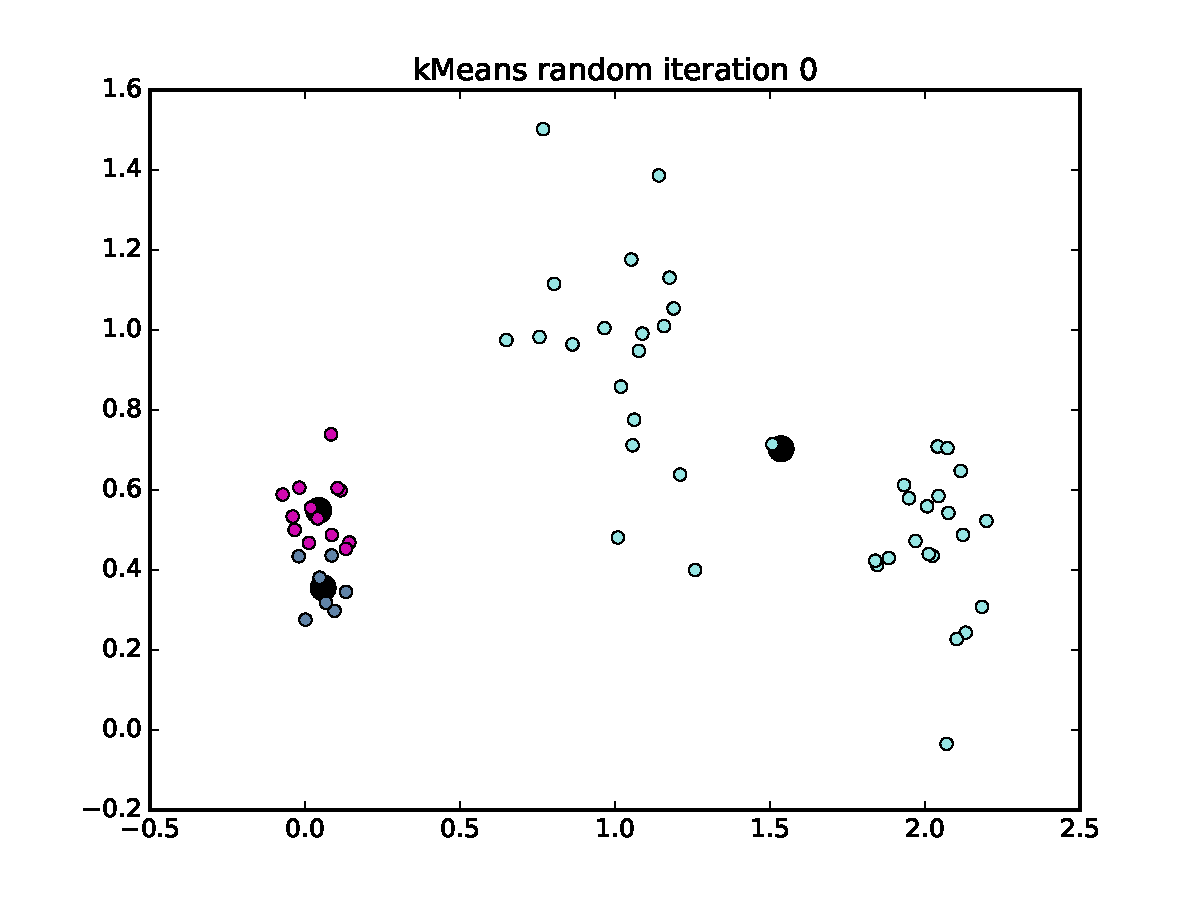
\includegraphics[width=0.45\textwidth]{kMeansrandomiteration0}
                        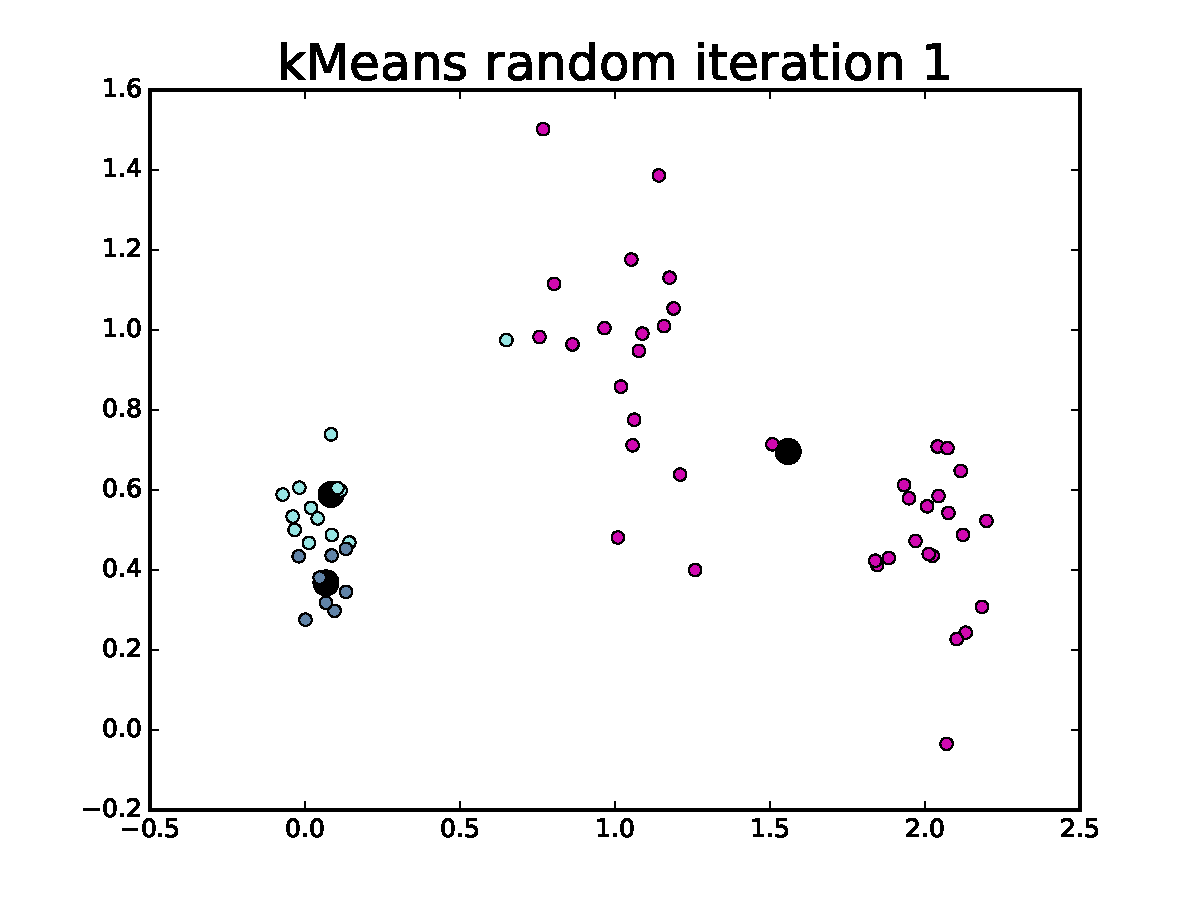
\includegraphics[width=0.45\textwidth]{kMeansrandomiteration1}
                        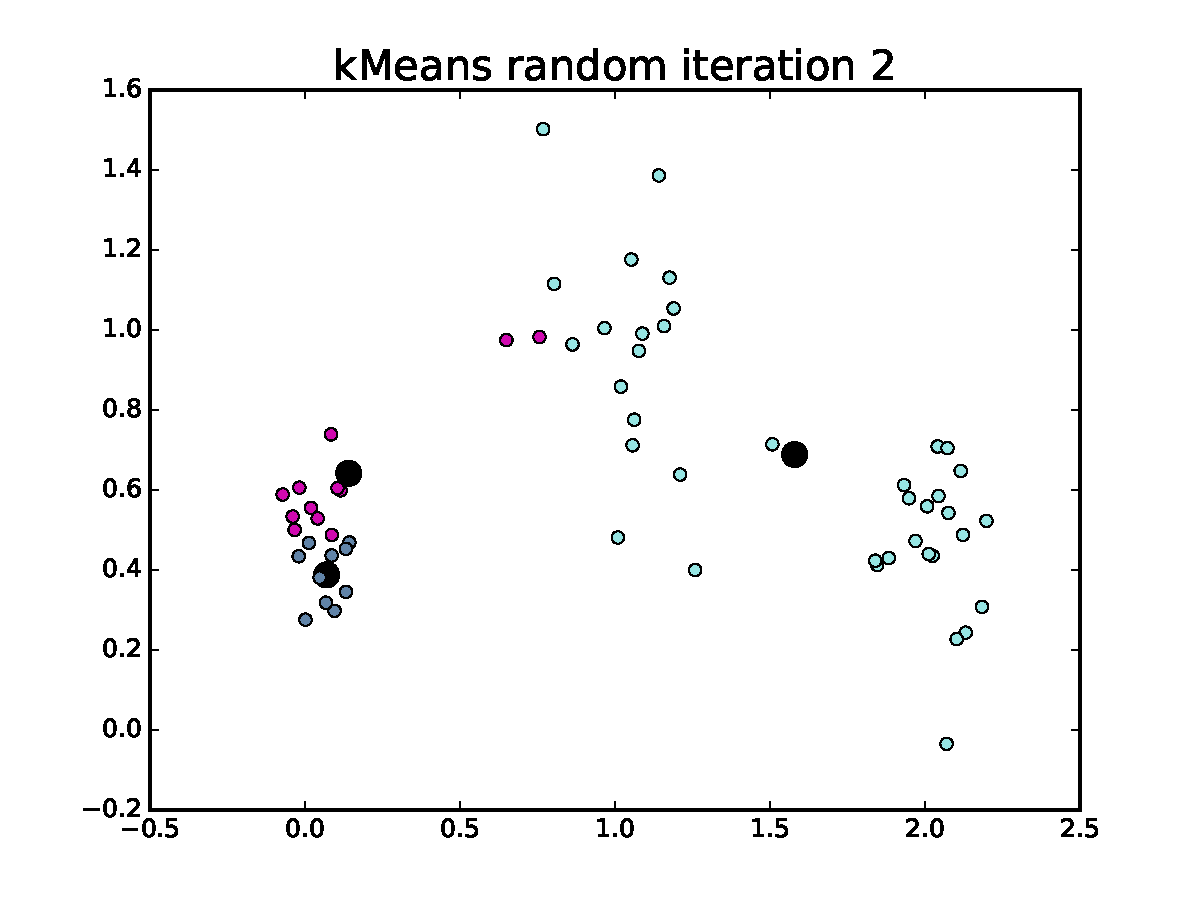
\includegraphics[width=0.45\textwidth]{kMeansrandomiteration2}
                        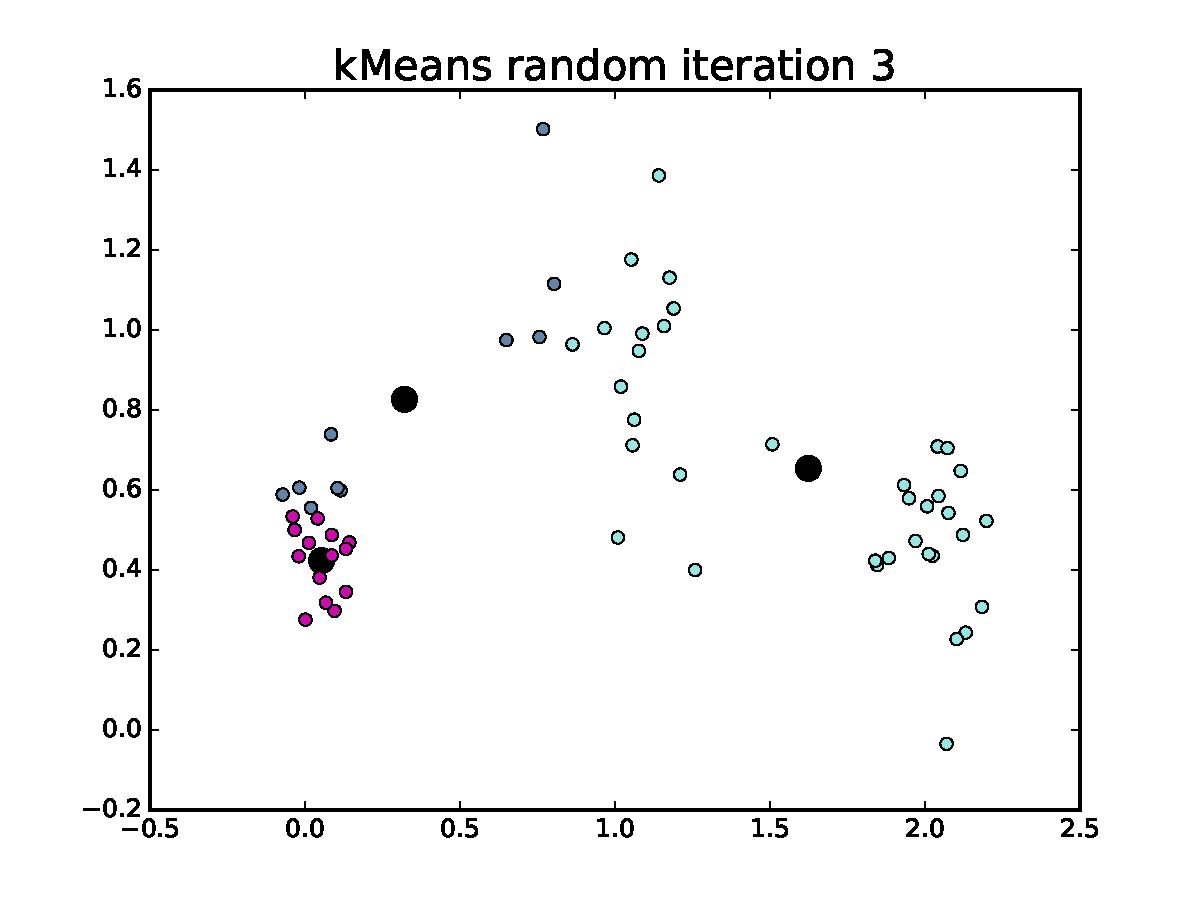
\includegraphics[width=0.45\textwidth]{kMeansrandomiteration3}
                        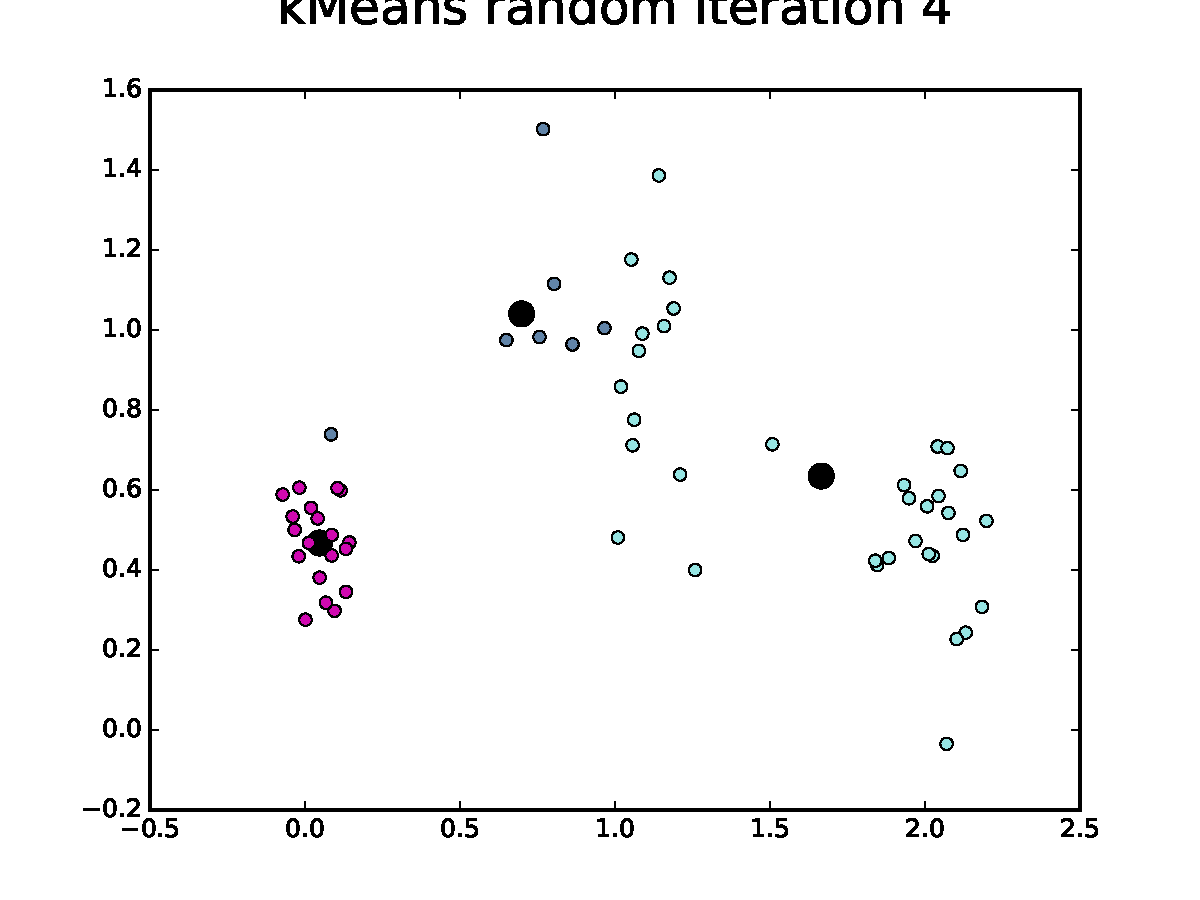
\includegraphics[width=0.45\textwidth]{kMeansrandomiteration4}
                        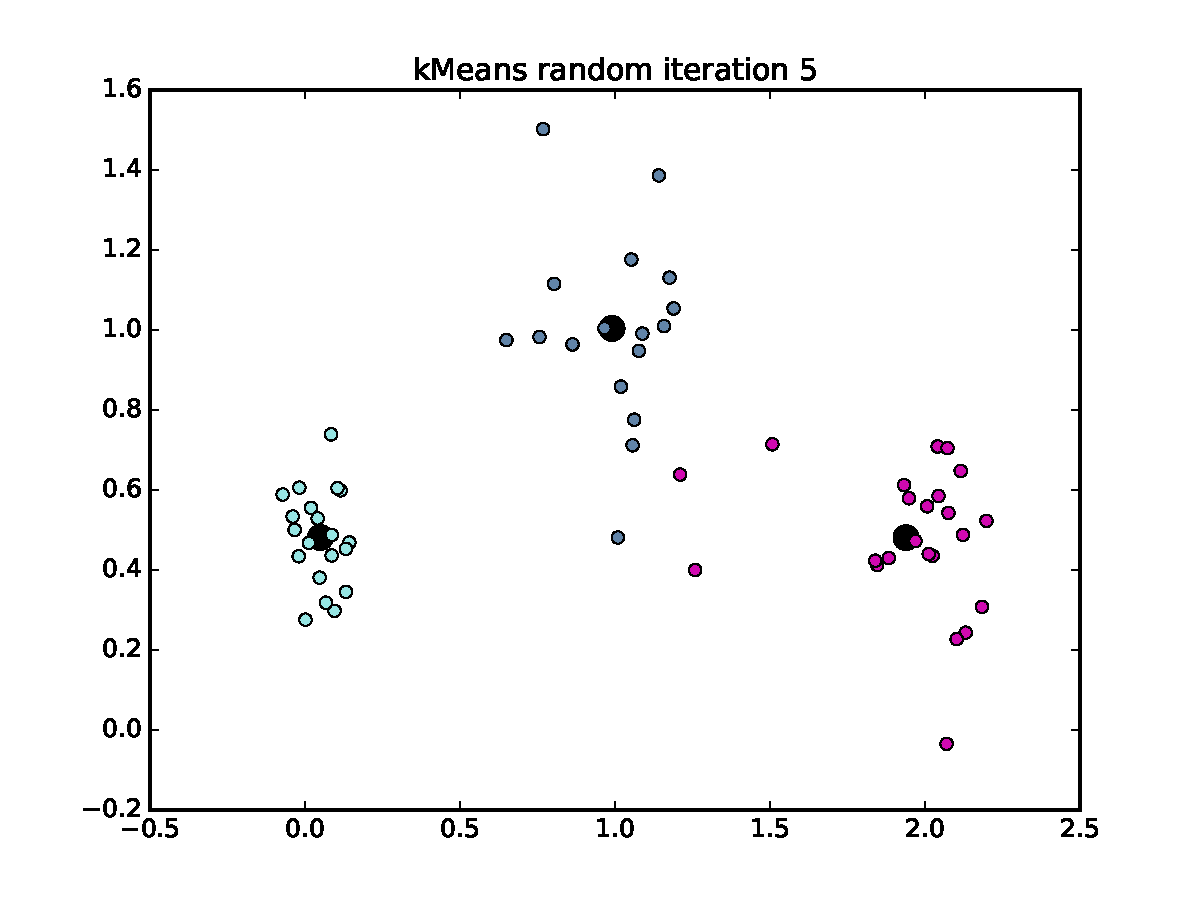
\includegraphics[width=0.45\textwidth]{kMeansrandomiteration5}
                        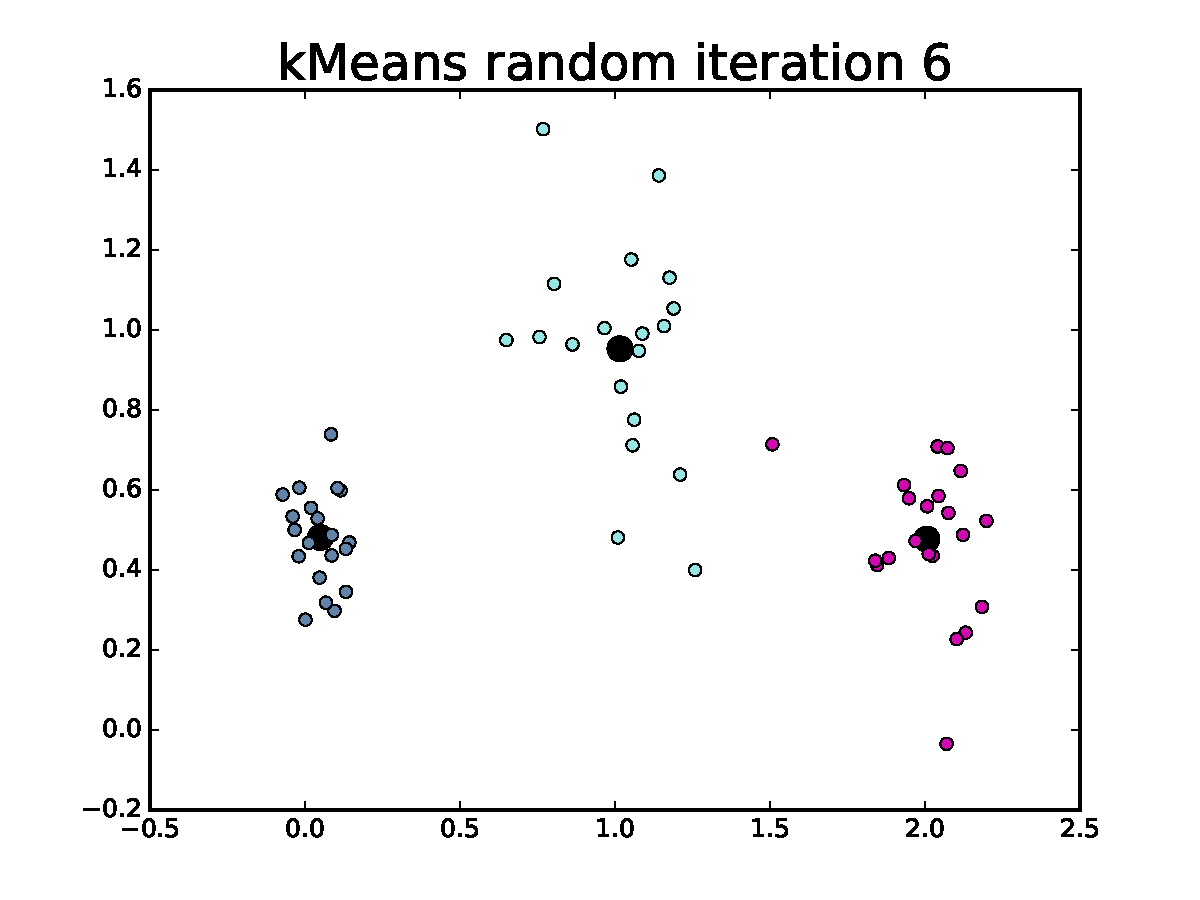
\includegraphics[width=0.45\textwidth]{kMeansrandomiteration6}
                        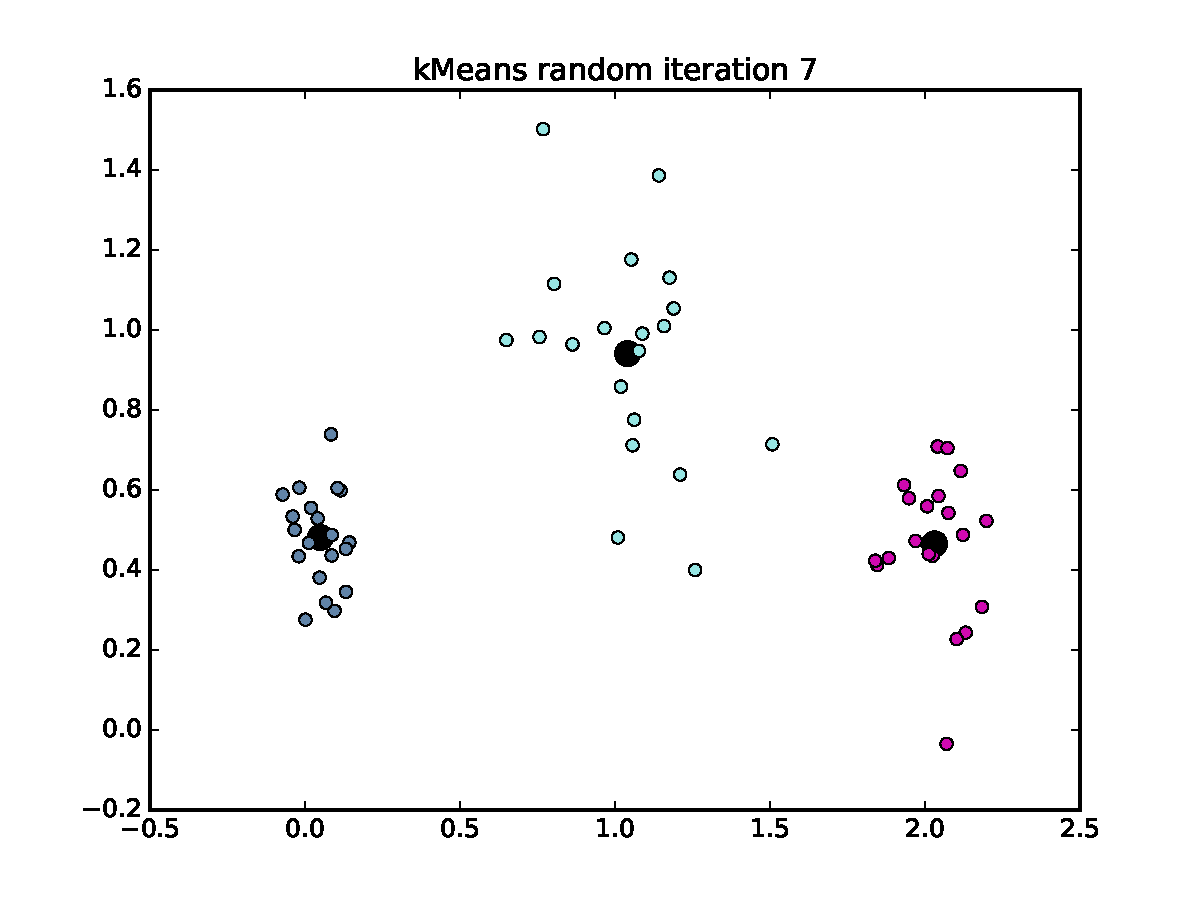
\includegraphics[width=0.45\textwidth]{kMeansrandomiteration7}
                        \caption{All iterations of kMeans with random initialization.}
                \end{center}
        \end{adjustwidth}
\end{figure}
\clearpage

\paragraph{e)}

The results of running the \texttt{kMedoids} algorithm with a random initialization are shown in the following figure.
\begin{figure}[h]
        \begin{adjustwidth}{-2in}{-2in}
                \begin{center}
                        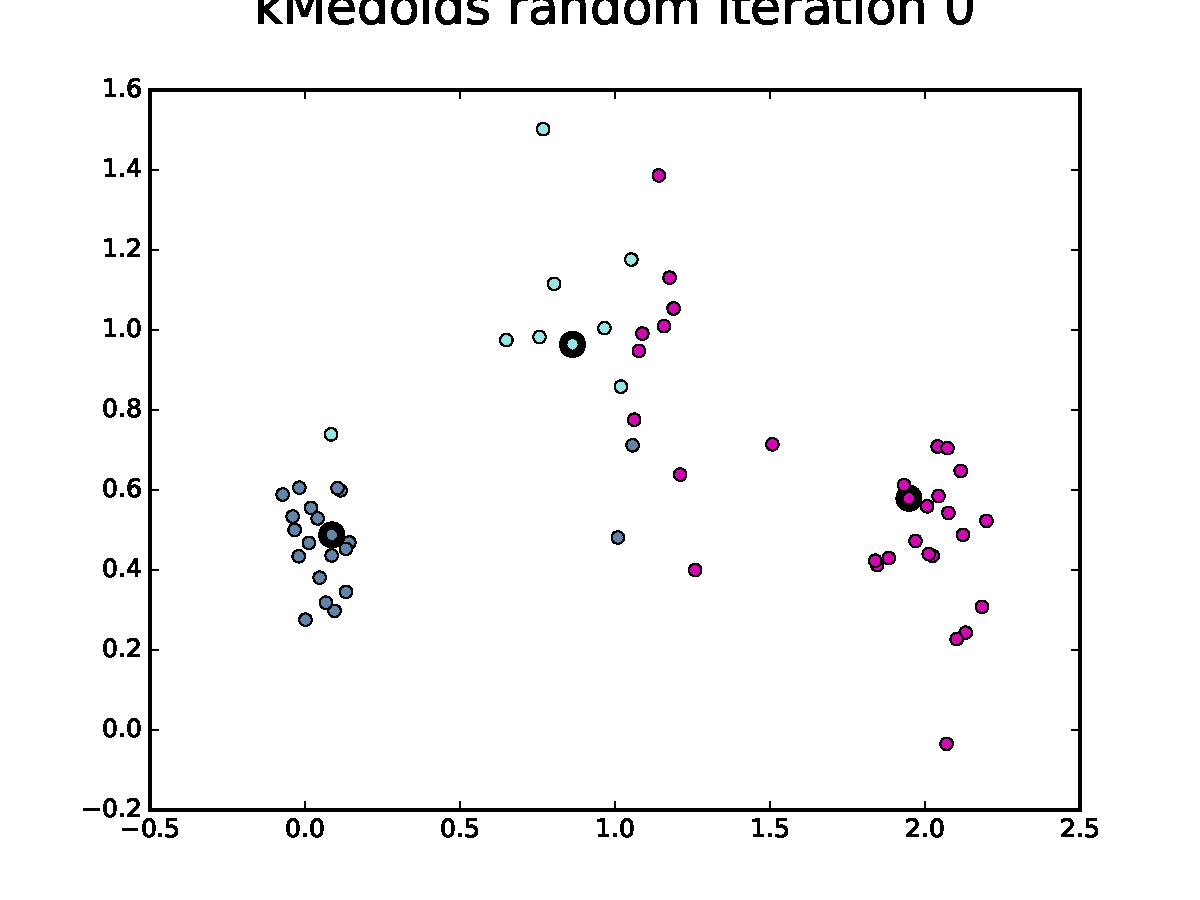
\includegraphics[width=0.45\textwidth]{kMedoidsrandomiteration0}
                        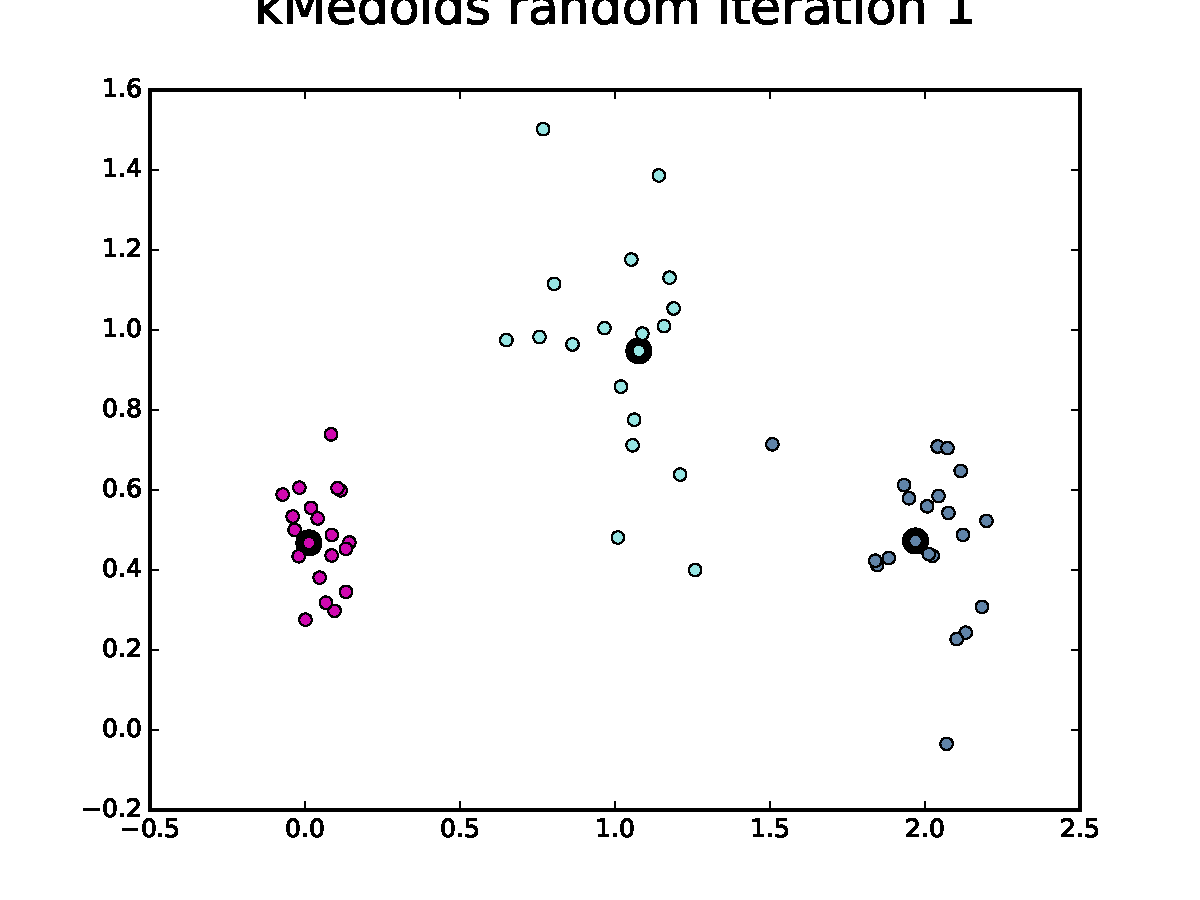
\includegraphics[width=0.45\textwidth]{kMedoidsrandomiteration1}
                        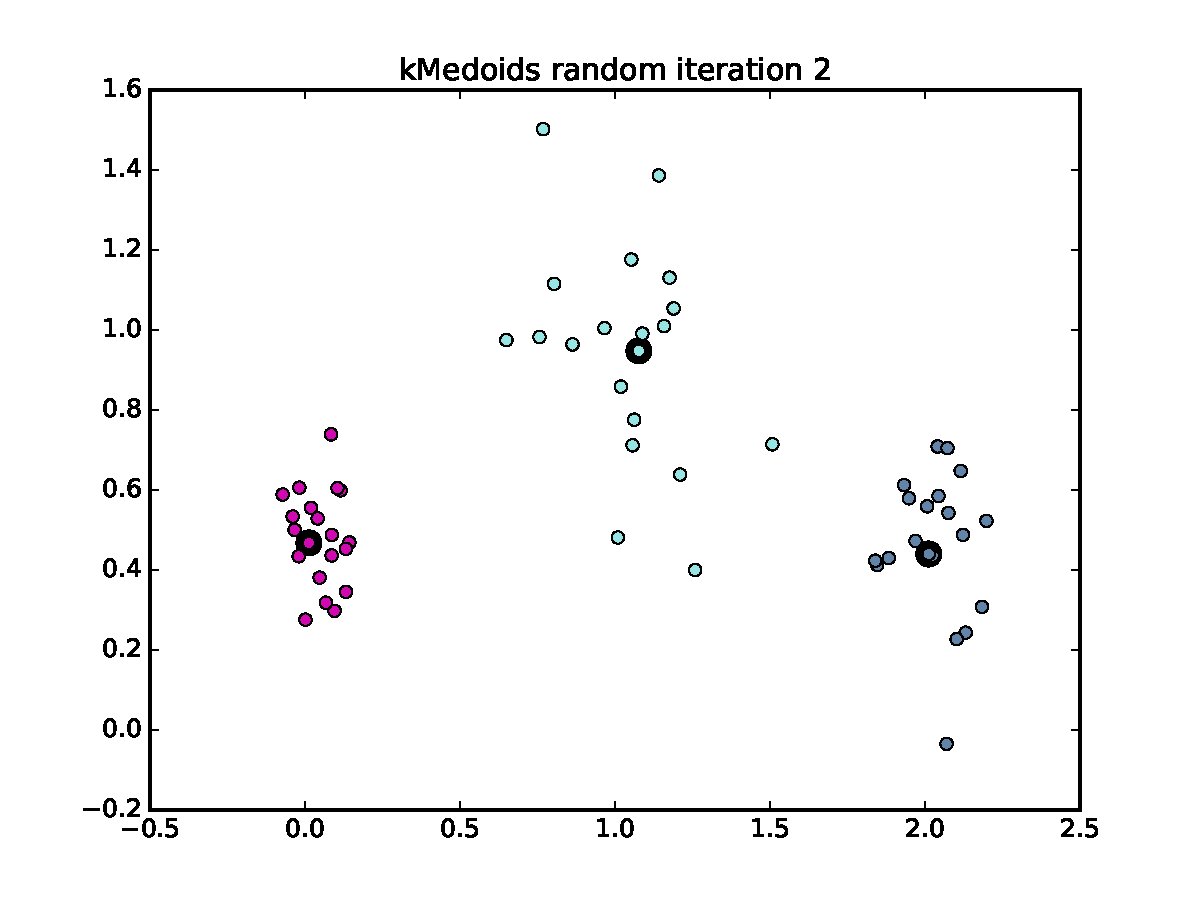
\includegraphics[width=0.45\textwidth]{kMedoidsrandomiteration2}
                        \caption{All iterations of kMedoids with random initialization.}
                \end{center}
        \end{adjustwidth}
\end{figure}

\paragraph{f)}

The results of running the \texttt{kMeans} and \texttt{kMedoids} algorithm with a cheating initialization are shown in the following figure.
\begin{figure}[h]
        \begin{center}
                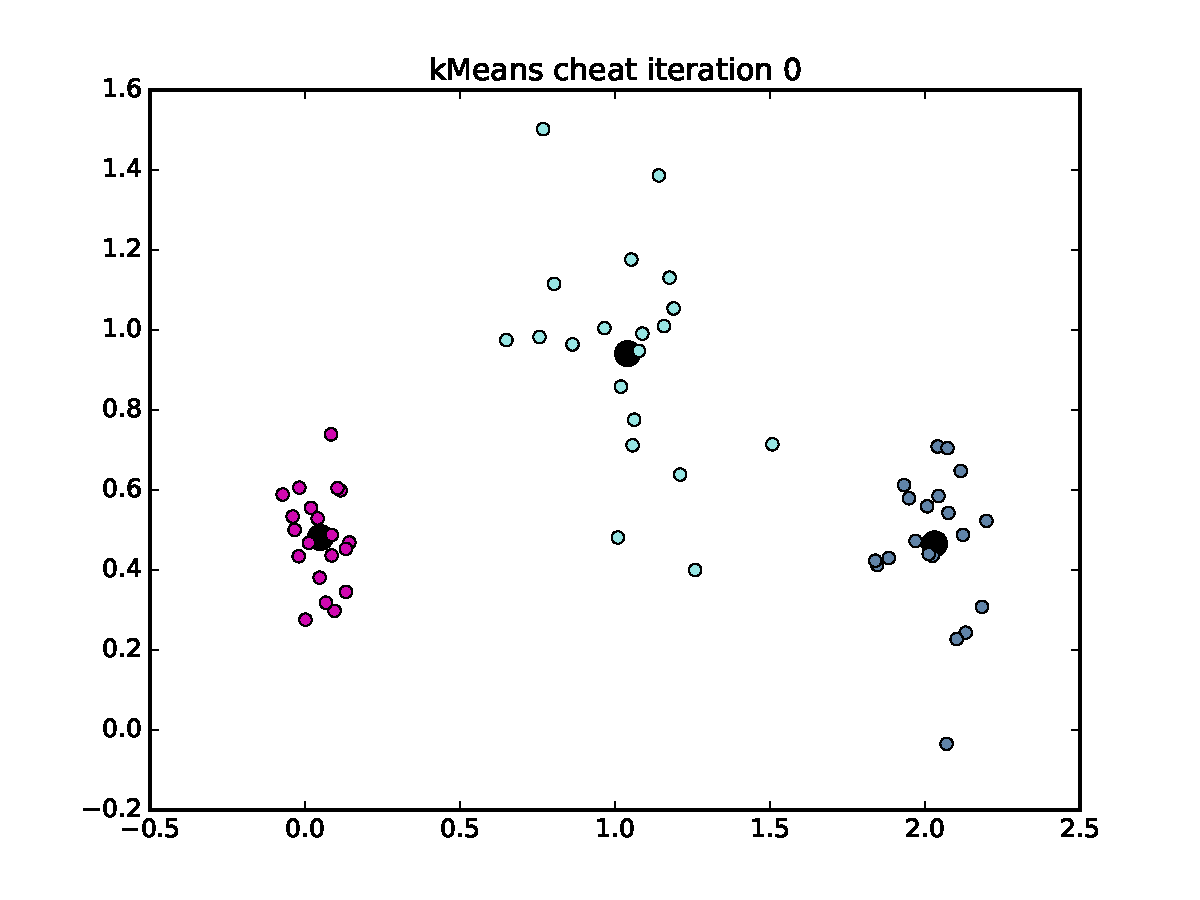
\includegraphics[width=0.495\textwidth]{kMeanscheatiteration0}
                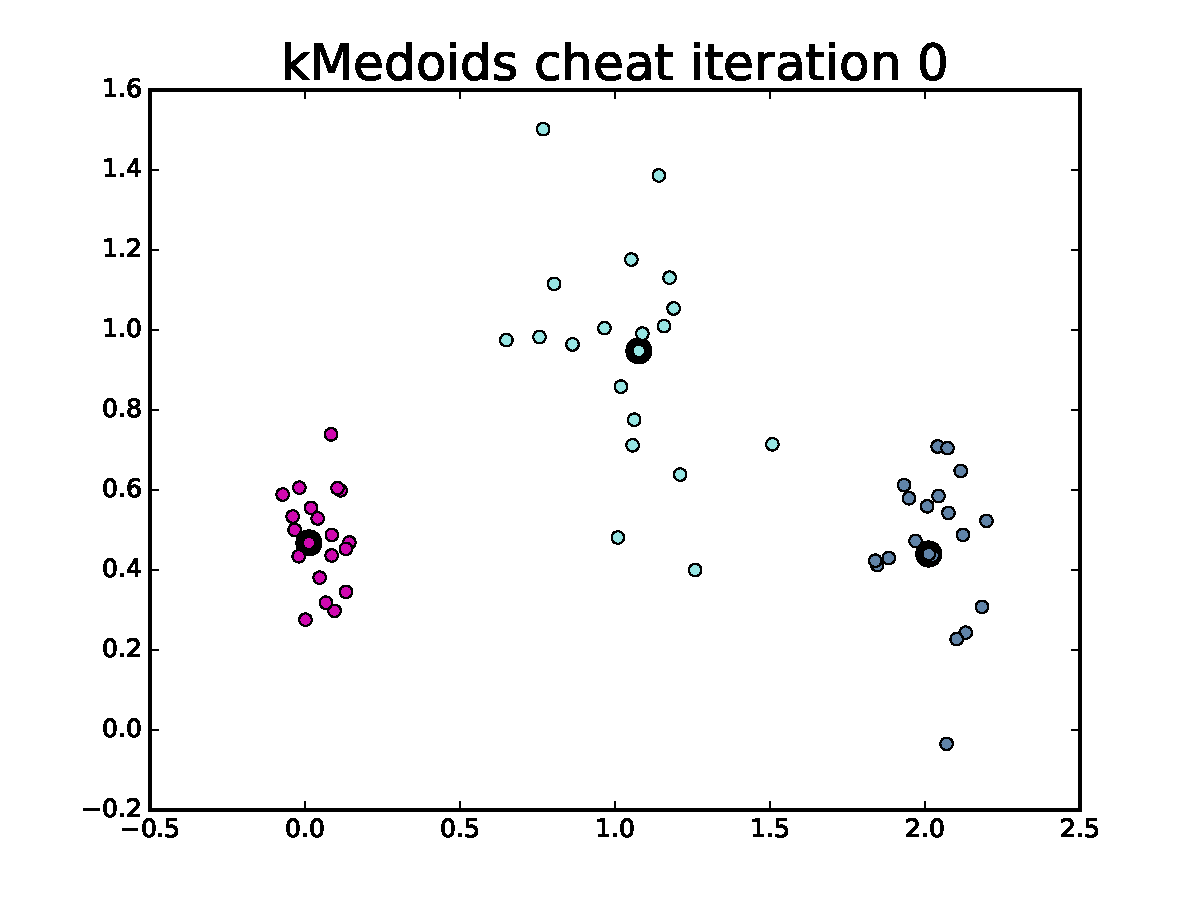
\includegraphics[width=0.495\textwidth]{kMedoidscheatiteration0}
                \caption{kMeans and kMedoids with cheating initialization.}
        \end{center}
\end{figure}
Note that both algorithms terminated after one iteration as the cheating allowed the algorithms to begin with the optimal clusters.

\end{document}